
        \documentclass[spanish, 11pt]{exam}

        %These tell TeX which packages to use.
        \usepackage{array,epsfig}
        \usepackage{amsmath, textcomp}
        \usepackage{amsfonts}
        \usepackage{amssymb}
        \usepackage{amsxtra}
        \usepackage{amsthm}
        \usepackage{mathrsfs}
        \usepackage{color}
        \usepackage{multicol, xparse}
        \usepackage{verbatim}


        \usepackage[utf8]{inputenc}
        \usepackage[spanish]{babel}
        \usepackage{eurosym}

        \usepackage{graphicx}
        \graphicspath{{../img/}}
        \usepackage{pgf}



        \printanswers
        \nopointsinmargin
        \pointformat{}

        %Pagination stuff.
        %\setlength{\topmargin}{-.3 in}
        %\setlength{\oddsidemargin}{0in}
        %\setlength{\evensidemargin}{0in}
        %\setlength{\textheight}{9.in}
        %\setlength{\textwidth}{6.5in}
        %\pagestyle{empty}

        \let\multicolmulticols\multicols
        \let\endmulticolmulticols\endmulticols
        \RenewDocumentEnvironment{multicols}{mO{}}
         {%
          \ifnum#1=1
            #2%
          \else % More than 1 column
            \multicolmulticols{#1}[#2]
          \fi
         }
         {%
          \ifnum#1=1
          \else % More than 1 column
            \endmulticolmulticols
          \fi
         }
        \renewcommand{\solutiontitle}{\noindent\textbf{Sol:}\enspace}

        \newcommand{\samedir}{\mathbin{\!/\mkern-5mu/\!}}

        \newcommand{\class}{1º Bachillerato}
        \newcommand{\examdate}{\today}

        \newcommand{\tipo}{A}


        \newcommand{\timelimit}{50 minutos}



        \pagestyle{head}
        \firstpageheader{
\includegraphics[width=0.2\columnwidth]{header_left}}{\textbf{Departamento de Matemáticas\linebreak \class}\linebreak \examnum}{
\includegraphics[width=0.1\columnwidth]{header_right}}
        \runningheader{\class}{\examnum}{Página \thepage\ of \numpages}
        \runningheadrule

        \newcommand{\examnum}{Autoevaluación de Estadística}
        \begin{document}
        \begin{questions}
        \question au0pe02 - Se realiza una encuesta a un grupo de 21 personas acerca del número de veces que acuden al cine a lo largo de un año, obteniéndose los siguientes resultados:4 2 6 8 3 4 3 5 7 1 3 4 5 7 2 2 1 3 12 5 4
        \begin{multicols}{1}
        \begin{parts} \part[1] Realiza una tabla de frecuencias  \begin{solution}   \begin{tabular}{rrrrrrr}
\hline
   x\_i &   f\_i &   F\_i &       h\_i &       H\_i &      \%\_i &      \%A\_i \\
\hline
     1 &     2 &     2 & 0.0952381 & 0.0952381 &  9.52381 &   9.52381 \\
     2 &     3 &     5 & 0.142857  & 0.238095  & 14.2857  &  23.8095  \\
     3 &     4 &     9 & 0.190476  & 0.428571  & 19.0476  &  42.8571  \\
     4 &     4 &    13 & 0.190476  & 0.619048  & 19.0476  &  61.9048  \\
     5 &     3 &    16 & 0.142857  & 0.761905  & 14.2857  &  76.1905  \\
     6 &     1 &    17 & 0.047619  & 0.809524  &  4.7619  &  80.9524  \\
     7 &     2 &    19 & 0.0952381 & 0.904762  &  9.52381 &  90.4762  \\
     8 &     1 &    20 & 0.047619  & 0.952381  &  4.7619  &  95.2381  \\
    12 &     1 &    21 & 0.047619  & 1         &  4.7619  & 100       \\
\hline
\end{tabular}   \end{solution} \part[1] Realiza un diagrama de barras y un polígono de frecuencias  \begin{solution}   \\ \resizebox {0.5\textwidth}{!}{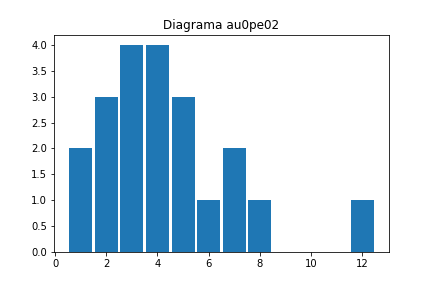
\includegraphics[width=1\columnwidth]{au0pe02}}   \end{solution} \part[1] Calcular los parámetros de centralización  \begin{solution}   {'media': 4.333333333333333, 'mediana': 4.0, 'moda': ModeResult(mode=array([3]), count=array([4]))}   \end{solution} \part[1] Calcular los parámetros de posición P70, Q1, Q3, D4  \begin{solution}   {'P70': 5.0, 'Q1': 3.0, 'Q3': 5.0, 'D4': 3.0}   \end{solution} \part[1] Calcular los parámetros de dispersión  \begin{solution}   {'rango': 11, 'varianza': 6.507936507936508, 'desviación típica': 2.55106575923407, 'coeficiente variación': 0.588707482900170}   \end{solution}
        \end{parts}
        \end{multicols}
        \question au2p090e07 - En una consulta médica la distribución de pacientes por su edad ha sido, en la última semana, la siguiente:\\\begin{tabular}{rlr}
\hline
    & Duración              &   Cantidad \\
\hline
  0 & $\left[15, 23\right)$ &          3 \\
  1 & $\left[23, 31\right)$ &          4 \\
  2 & $\left[31, 39\right)$ &          5 \\
  3 & $\left[39, 47\right)$ &          8 \\
  4 & $\left[47, 55\right)$ &         10 \\
  5 & $\left[55, 63\right)$ &         12 \\
  6 & $\left[63, 71\right)$ &         15 \\
  7 & $\left[71, 79\right)$ &         12 \\
  8 & $\left[79, 87\right)$ &          6 \\
\hline
\end{tabular}
        \begin{multicols}{1}
        \begin{parts} \part[1] Haz una tabla de frecuencias  \begin{solution}   \begin{tabular}{rrrrrrrrrr}
\hline
    &   lim\_inf &   lim\_sup &   x\_i &   f\_i &   F\_i &       h\_i &         H\_i &   x\_if\_i &   x\^{}2\_if\_i \\
\hline
  0 &        15 &        23 &    19 &     3 &     3 & 0.04      &   0.04      &       57 &       1083 \\
  1 &        23 &        31 &    27 &     4 &     7 & 0.0533333 &   0.0933333 &      108 &       2916 \\
  2 &        31 &        39 &    35 &     5 &    12 & 0.0666667 &   0.16      &      175 &       6125 \\
  3 &        39 &        47 &    43 &     8 &    20 & 0.106667  &   0.266667  &      344 &      14792 \\
  4 &        47 &        55 &    51 &    10 &    30 & 0.133333  &   0.4       &      510 &      26010 \\
  5 &        55 &        63 &    59 &    12 &    42 & 0.16      &   0.56      &      708 &      41772 \\
  6 &        63 &        71 &    67 &    15 &    57 & 0.2       &   0.76      &     1005 &      67335 \\
  7 &        71 &        79 &    75 &    12 &    69 & 0.16      &   0.92      &      900 &      67500 \\
  8 &        79 &        87 &    83 &     6 &    75 & 0.08      &   1         &      498 &      41334 \\
  9 &       nan &       nan &   nan &    75 &   nan & 1         & nan         &     4305 &     268867 \\
\hline
\end{tabular}   \end{solution} \part[1] Calcula media, la varianza, la desviación típica y el coeficiente de variación  \begin{solution}   {'media': 57.4, 'varianza': 290.13333333333367, 'desviación típica': 17.0333007175161, 'coeficiente de variación': 0.296747399259862}   \end{solution} \part[1] La edad mas frecuente de los pacientes  \begin{solution}   {'Intervalo modal': '$\\left[63.0, 71.0\\right)$', 'moda': 67.0}   \end{solution} \part[1] El percentil 47  \begin{solution}   {'k': 47, 'N': 75.0, '$L_i$': 55.0, '$f_i$': 12.0, '$F_{i-1}$': 30.0, '$C_i$': 8.0, 'percentil': 58.5}   \end{solution} \part[1] ¿Qué porcentaje de pacientes tenían una edad superior a 60 años?  \begin{solution}   {'valor': 60, 'N': 75.0, '$L_i$': 55.0, '$f_i$': 12.0, '$F_{i-1}$': 30.0, '$C_i$': 8.0, 'Porcentaje': 50.0000000000000}   \end{solution}
        \end{parts}
        \end{multicols}
        \question au3e1 - Una oficina bancaría ha tabulado las cantidades de dinero que retiran de sus cuentas 100 clientes jóvenes en
un determinado día:\\\begin{tabular}{rlr}
\hline
    & Duración               &   Cantidad \\
\hline
  0 & $\left[0, 40\right)$   &         40 \\
  1 & $\left[40, 80\right)$  &         35 \\
  2 & $\left[80, 120\right)$ &         25 \\
\hline
\end{tabular}
        \begin{multicols}{1}
        \begin{parts} \part[1] Realizar una tabla de frecuencias con los datos que vayas a necesitar para resolver el ejercicio  \begin{solution}   \begin{tabular}{rrrrrrrrrr}
\hline
    &   lim\_inf &   lim\_sup &   x\_i &   f\_i &   F\_i &   h\_i &    H\_i &   x\_if\_i &   x\^{}2\_if\_i \\
\hline
  0 &         0 &        40 &    20 &    40 &    40 &  0.4  &   0.4  &      800 &      16000 \\
  1 &        40 &        80 &    60 &    35 &    75 &  0.35 &   0.75 &     2100 &     126000 \\
  2 &        80 &       120 &   100 &    25 &   100 &  0.25 &   1    &     2500 &     250000 \\
  3 &       nan &       nan &   nan &   100 &   nan &  1    & nan    &     5400 &     392000 \\
\hline
\end{tabular}   \end{solution} \part[1] Calcula media, la varianza, la desviación típica y el coeficiente de variación  \begin{solution}   {'media': 54.0, 'varianza': 1004.0, 'desviación típica': 31.6859590355097, 'coeficiente de variación': 0.586777019176106}   \end{solution} \part[1] La mediana  \begin{solution}   {'k': 50, 'N': 100.0, '$L_i$': 40.0, '$f_i$': 35.0, '$F_{i-1}$': 40.0, '$C_i$': 40.0, 'percentil': 51.42857142857143}   \end{solution} \part[1] El percentil 70  \begin{solution}   {'k': 70, 'N': 100.0, '$L_i$': 40.0, '$f_i$': 35.0, '$F_{i-1}$': 40.0, '$C_i$': 40.0, 'percentil': 74.28571428571428}   \end{solution} \part[1] ¿Qué porcentaje de clientes ha retirado menos de 60 \euro?  \begin{solution}   {'valor': 60, 'N': 100.0, '$L_i$': 40.0, '$f_i$': 35.0, '$F_{i-1}$': 40.0, '$C_i$': 40.0, 'Porcentaje': 57.5000000000000}   \end{solution}
        \end{parts}
        \end{multicols}
        \question au4p093e05 - La temperatura media en los meses de invierno en varias ciudades y el gasto medio por habitante en
calefacción ha sido\\\begin{tabular}{lrrrrrr}
\hline
                      &   0 &   1 &   2 &   3 &   4 &   5 \\
\hline
 Temperatura (grados) &  10 &  12 &  14 &  15 &  17 &  20 \\
 Gasto (euros)        & 150 & 120 & 102 &  90 &  50 &  18 \\
\hline
\end{tabular}
        \begin{multicols}{1}
        \begin{parts} \part[1] Haz una tabla de frecuencias con los datos que necesites para hace el resto de apartados  \begin{solution}   \begin{tabular}{rrrrrr}
\hline
    &   x &   y &   xy &   x2 &    y2 \\
\hline
  0 &  10 & 150 & 1500 &  100 & 22500 \\
  1 &  12 & 120 & 1440 &  144 & 14400 \\
  2 &  14 & 102 & 1428 &  196 & 10404 \\
  3 &  15 &  90 & 1350 &  225 &  8100 \\
  4 &  17 &  50 &  850 &  289 &  2500 \\
  5 &  20 &  18 &  360 &  400 &   324 \\
  6 &  88 & 530 & 6928 & 1354 & 58228 \\
\hline
\end{tabular}   \end{solution} \part[1] Calcula el gasto medio  \begin{solution}   {'media': 88.33333333333333}   \end{solution} \part[1] Halla el coeficiente de correlación lineal e interprétalo  \begin{solution}   {'media de x': 14.666666666666666, 'desviación de x': 3.2489314482696545, 'media de y': 88.33333333333333, 'desviación de y': 43.61065109453067, 'covarianza': -140.88888888888889, 'coeficiente de correlación': -0.9943599539663297}   \end{solution} \part[1] Estima el gasto medio por habitante de una ciudad si la temperatura media hubiera sido 8ºC  \begin{solution}   $y = - 13.3473684210526 x + 284.094736842105$ \\\resizebox {0.5\textwidth}{!}{%% Creator: Matplotlib, PGF backend
%%
%% To include the figure in your LaTeX document, write
%%   \input{<filename>.pgf}
%%
%% Make sure the required packages are loaded in your preamble
%%   \usepackage{pgf}
%%
%% Figures using additional raster images can only be included by \input if
%% they are in the same directory as the main LaTeX file. For loading figures
%% from other directories you can use the `import` package
%%   \usepackage{import}
%% and then include the figures with
%%   \import{<path to file>}{<filename>.pgf}
%%
%% Matplotlib used the following preamble
%%   \usepackage{fontspec}
%%   \setmainfont{DejaVuSerif.ttf}[Path=/home/hp/Mis_aplicaciones/anaconda3/lib/python3.6/site-packages/matplotlib/mpl-data/fonts/ttf/]
%%   \setsansfont{DejaVuSans.ttf}[Path=/home/hp/Mis_aplicaciones/anaconda3/lib/python3.6/site-packages/matplotlib/mpl-data/fonts/ttf/]
%%   \setmonofont{DejaVuSansMono.ttf}[Path=/home/hp/Mis_aplicaciones/anaconda3/lib/python3.6/site-packages/matplotlib/mpl-data/fonts/ttf/]
%%
\begingroup%
\makeatletter%
\begin{pgfpicture}%
\pgfpathrectangle{\pgfpointorigin}{\pgfqpoint{6.000000in}{4.000000in}}%
\pgfusepath{use as bounding box, clip}%
\begin{pgfscope}%
\pgfsetbuttcap%
\pgfsetmiterjoin%
\definecolor{currentfill}{rgb}{1.000000,1.000000,1.000000}%
\pgfsetfillcolor{currentfill}%
\pgfsetlinewidth{0.000000pt}%
\definecolor{currentstroke}{rgb}{1.000000,1.000000,1.000000}%
\pgfsetstrokecolor{currentstroke}%
\pgfsetdash{}{0pt}%
\pgfpathmoveto{\pgfqpoint{0.000000in}{0.000000in}}%
\pgfpathlineto{\pgfqpoint{6.000000in}{0.000000in}}%
\pgfpathlineto{\pgfqpoint{6.000000in}{4.000000in}}%
\pgfpathlineto{\pgfqpoint{0.000000in}{4.000000in}}%
\pgfpathclose%
\pgfusepath{fill}%
\end{pgfscope}%
\begin{pgfscope}%
\pgfsetbuttcap%
\pgfsetmiterjoin%
\definecolor{currentfill}{rgb}{1.000000,1.000000,1.000000}%
\pgfsetfillcolor{currentfill}%
\pgfsetlinewidth{0.000000pt}%
\definecolor{currentstroke}{rgb}{0.000000,0.000000,0.000000}%
\pgfsetstrokecolor{currentstroke}%
\pgfsetstrokeopacity{0.000000}%
\pgfsetdash{}{0pt}%
\pgfpathmoveto{\pgfqpoint{0.750000in}{0.500000in}}%
\pgfpathlineto{\pgfqpoint{5.400000in}{0.500000in}}%
\pgfpathlineto{\pgfqpoint{5.400000in}{3.520000in}}%
\pgfpathlineto{\pgfqpoint{0.750000in}{3.520000in}}%
\pgfpathclose%
\pgfusepath{fill}%
\end{pgfscope}%
\begin{pgfscope}%
\pgfpathrectangle{\pgfqpoint{0.750000in}{0.500000in}}{\pgfqpoint{4.650000in}{3.020000in}}%
\pgfusepath{clip}%
\pgfsetbuttcap%
\pgfsetroundjoin%
\definecolor{currentfill}{rgb}{0.121569,0.466667,0.705882}%
\pgfsetfillcolor{currentfill}%
\pgfsetfillopacity{0.800000}%
\pgfsetlinewidth{1.003750pt}%
\definecolor{currentstroke}{rgb}{0.121569,0.466667,0.705882}%
\pgfsetstrokecolor{currentstroke}%
\pgfsetstrokeopacity{0.800000}%
\pgfsetdash{}{0pt}%
\pgfpathmoveto{\pgfqpoint{0.967457in}{3.053442in}}%
\pgfpathcurveto{\pgfqpoint{0.978507in}{3.053442in}}{\pgfqpoint{0.989106in}{3.057832in}}{\pgfqpoint{0.996920in}{3.065646in}}%
\pgfpathcurveto{\pgfqpoint{1.004734in}{3.073459in}}{\pgfqpoint{1.009124in}{3.084058in}}{\pgfqpoint{1.009124in}{3.095108in}}%
\pgfpathcurveto{\pgfqpoint{1.009124in}{3.106159in}}{\pgfqpoint{1.004734in}{3.116758in}}{\pgfqpoint{0.996920in}{3.124571in}}%
\pgfpathcurveto{\pgfqpoint{0.989106in}{3.132385in}}{\pgfqpoint{0.978507in}{3.136775in}}{\pgfqpoint{0.967457in}{3.136775in}}%
\pgfpathcurveto{\pgfqpoint{0.956407in}{3.136775in}}{\pgfqpoint{0.945808in}{3.132385in}}{\pgfqpoint{0.937994in}{3.124571in}}%
\pgfpathcurveto{\pgfqpoint{0.930181in}{3.116758in}}{\pgfqpoint{0.925790in}{3.106159in}}{\pgfqpoint{0.925790in}{3.095108in}}%
\pgfpathcurveto{\pgfqpoint{0.925790in}{3.084058in}}{\pgfqpoint{0.930181in}{3.073459in}}{\pgfqpoint{0.937994in}{3.065646in}}%
\pgfpathcurveto{\pgfqpoint{0.945808in}{3.057832in}}{\pgfqpoint{0.956407in}{3.053442in}}{\pgfqpoint{0.967457in}{3.053442in}}%
\pgfpathclose%
\pgfusepath{stroke,fill}%
\end{pgfscope}%
\begin{pgfscope}%
\pgfpathrectangle{\pgfqpoint{0.750000in}{0.500000in}}{\pgfqpoint{4.650000in}{3.020000in}}%
\pgfusepath{clip}%
\pgfsetbuttcap%
\pgfsetroundjoin%
\definecolor{currentfill}{rgb}{0.121569,0.466667,0.705882}%
\pgfsetfillcolor{currentfill}%
\pgfsetfillopacity{0.800000}%
\pgfsetlinewidth{1.003750pt}%
\definecolor{currentstroke}{rgb}{0.121569,0.466667,0.705882}%
\pgfsetstrokecolor{currentstroke}%
\pgfsetstrokeopacity{0.800000}%
\pgfsetdash{}{0pt}%
\pgfpathmoveto{\pgfqpoint{1.810474in}{2.562622in}}%
\pgfpathcurveto{\pgfqpoint{1.821524in}{2.562622in}}{\pgfqpoint{1.832123in}{2.567012in}}{\pgfqpoint{1.839937in}{2.574826in}}%
\pgfpathcurveto{\pgfqpoint{1.847751in}{2.582639in}}{\pgfqpoint{1.852141in}{2.593238in}}{\pgfqpoint{1.852141in}{2.604288in}}%
\pgfpathcurveto{\pgfqpoint{1.852141in}{2.615339in}}{\pgfqpoint{1.847751in}{2.625938in}}{\pgfqpoint{1.839937in}{2.633751in}}%
\pgfpathcurveto{\pgfqpoint{1.832123in}{2.641565in}}{\pgfqpoint{1.821524in}{2.645955in}}{\pgfqpoint{1.810474in}{2.645955in}}%
\pgfpathcurveto{\pgfqpoint{1.799424in}{2.645955in}}{\pgfqpoint{1.788825in}{2.641565in}}{\pgfqpoint{1.781011in}{2.633751in}}%
\pgfpathcurveto{\pgfqpoint{1.773198in}{2.625938in}}{\pgfqpoint{1.768808in}{2.615339in}}{\pgfqpoint{1.768808in}{2.604288in}}%
\pgfpathcurveto{\pgfqpoint{1.768808in}{2.593238in}}{\pgfqpoint{1.773198in}{2.582639in}}{\pgfqpoint{1.781011in}{2.574826in}}%
\pgfpathcurveto{\pgfqpoint{1.788825in}{2.567012in}}{\pgfqpoint{1.799424in}{2.562622in}}{\pgfqpoint{1.810474in}{2.562622in}}%
\pgfpathclose%
\pgfusepath{stroke,fill}%
\end{pgfscope}%
\begin{pgfscope}%
\pgfpathrectangle{\pgfqpoint{0.750000in}{0.500000in}}{\pgfqpoint{4.650000in}{3.020000in}}%
\pgfusepath{clip}%
\pgfsetbuttcap%
\pgfsetroundjoin%
\definecolor{currentfill}{rgb}{0.121569,0.466667,0.705882}%
\pgfsetfillcolor{currentfill}%
\pgfsetfillopacity{0.800000}%
\pgfsetlinewidth{1.003750pt}%
\definecolor{currentstroke}{rgb}{0.121569,0.466667,0.705882}%
\pgfsetstrokecolor{currentstroke}%
\pgfsetstrokeopacity{0.800000}%
\pgfsetdash{}{0pt}%
\pgfpathmoveto{\pgfqpoint{2.653491in}{2.268130in}}%
\pgfpathcurveto{\pgfqpoint{2.664542in}{2.268130in}}{\pgfqpoint{2.675141in}{2.272520in}}{\pgfqpoint{2.682954in}{2.280334in}}%
\pgfpathcurveto{\pgfqpoint{2.690768in}{2.288147in}}{\pgfqpoint{2.695158in}{2.298746in}}{\pgfqpoint{2.695158in}{2.309796in}}%
\pgfpathcurveto{\pgfqpoint{2.695158in}{2.320847in}}{\pgfqpoint{2.690768in}{2.331446in}}{\pgfqpoint{2.682954in}{2.339259in}}%
\pgfpathcurveto{\pgfqpoint{2.675141in}{2.347073in}}{\pgfqpoint{2.664542in}{2.351463in}}{\pgfqpoint{2.653491in}{2.351463in}}%
\pgfpathcurveto{\pgfqpoint{2.642441in}{2.351463in}}{\pgfqpoint{2.631842in}{2.347073in}}{\pgfqpoint{2.624029in}{2.339259in}}%
\pgfpathcurveto{\pgfqpoint{2.616215in}{2.331446in}}{\pgfqpoint{2.611825in}{2.320847in}}{\pgfqpoint{2.611825in}{2.309796in}}%
\pgfpathcurveto{\pgfqpoint{2.611825in}{2.298746in}}{\pgfqpoint{2.616215in}{2.288147in}}{\pgfqpoint{2.624029in}{2.280334in}}%
\pgfpathcurveto{\pgfqpoint{2.631842in}{2.272520in}}{\pgfqpoint{2.642441in}{2.268130in}}{\pgfqpoint{2.653491in}{2.268130in}}%
\pgfpathclose%
\pgfusepath{stroke,fill}%
\end{pgfscope}%
\begin{pgfscope}%
\pgfpathrectangle{\pgfqpoint{0.750000in}{0.500000in}}{\pgfqpoint{4.650000in}{3.020000in}}%
\pgfusepath{clip}%
\pgfsetbuttcap%
\pgfsetroundjoin%
\definecolor{currentfill}{rgb}{0.121569,0.466667,0.705882}%
\pgfsetfillcolor{currentfill}%
\pgfsetfillopacity{0.800000}%
\pgfsetlinewidth{1.003750pt}%
\definecolor{currentstroke}{rgb}{0.121569,0.466667,0.705882}%
\pgfsetstrokecolor{currentstroke}%
\pgfsetstrokeopacity{0.800000}%
\pgfsetdash{}{0pt}%
\pgfpathmoveto{\pgfqpoint{3.075000in}{2.071802in}}%
\pgfpathcurveto{\pgfqpoint{3.086050in}{2.071802in}}{\pgfqpoint{3.096649in}{2.076192in}}{\pgfqpoint{3.104463in}{2.084006in}}%
\pgfpathcurveto{\pgfqpoint{3.112276in}{2.091819in}}{\pgfqpoint{3.116667in}{2.102418in}}{\pgfqpoint{3.116667in}{2.113468in}}%
\pgfpathcurveto{\pgfqpoint{3.116667in}{2.124519in}}{\pgfqpoint{3.112276in}{2.135118in}}{\pgfqpoint{3.104463in}{2.142931in}}%
\pgfpathcurveto{\pgfqpoint{3.096649in}{2.150745in}}{\pgfqpoint{3.086050in}{2.155135in}}{\pgfqpoint{3.075000in}{2.155135in}}%
\pgfpathcurveto{\pgfqpoint{3.063950in}{2.155135in}}{\pgfqpoint{3.053351in}{2.150745in}}{\pgfqpoint{3.045537in}{2.142931in}}%
\pgfpathcurveto{\pgfqpoint{3.037724in}{2.135118in}}{\pgfqpoint{3.033333in}{2.124519in}}{\pgfqpoint{3.033333in}{2.113468in}}%
\pgfpathcurveto{\pgfqpoint{3.033333in}{2.102418in}}{\pgfqpoint{3.037724in}{2.091819in}}{\pgfqpoint{3.045537in}{2.084006in}}%
\pgfpathcurveto{\pgfqpoint{3.053351in}{2.076192in}}{\pgfqpoint{3.063950in}{2.071802in}}{\pgfqpoint{3.075000in}{2.071802in}}%
\pgfpathclose%
\pgfusepath{stroke,fill}%
\end{pgfscope}%
\begin{pgfscope}%
\pgfpathrectangle{\pgfqpoint{0.750000in}{0.500000in}}{\pgfqpoint{4.650000in}{3.020000in}}%
\pgfusepath{clip}%
\pgfsetbuttcap%
\pgfsetroundjoin%
\definecolor{currentfill}{rgb}{0.121569,0.466667,0.705882}%
\pgfsetfillcolor{currentfill}%
\pgfsetfillopacity{0.800000}%
\pgfsetlinewidth{1.003750pt}%
\definecolor{currentstroke}{rgb}{0.121569,0.466667,0.705882}%
\pgfsetstrokecolor{currentstroke}%
\pgfsetstrokeopacity{0.800000}%
\pgfsetdash{}{0pt}%
\pgfpathmoveto{\pgfqpoint{3.918017in}{1.417375in}}%
\pgfpathcurveto{\pgfqpoint{3.929067in}{1.417375in}}{\pgfqpoint{3.939666in}{1.421765in}}{\pgfqpoint{3.947480in}{1.429579in}}%
\pgfpathcurveto{\pgfqpoint{3.955294in}{1.437393in}}{\pgfqpoint{3.959684in}{1.447992in}}{\pgfqpoint{3.959684in}{1.459042in}}%
\pgfpathcurveto{\pgfqpoint{3.959684in}{1.470092in}}{\pgfqpoint{3.955294in}{1.480691in}}{\pgfqpoint{3.947480in}{1.488505in}}%
\pgfpathcurveto{\pgfqpoint{3.939666in}{1.496318in}}{\pgfqpoint{3.929067in}{1.500708in}}{\pgfqpoint{3.918017in}{1.500708in}}%
\pgfpathcurveto{\pgfqpoint{3.906967in}{1.500708in}}{\pgfqpoint{3.896368in}{1.496318in}}{\pgfqpoint{3.888554in}{1.488505in}}%
\pgfpathcurveto{\pgfqpoint{3.880741in}{1.480691in}}{\pgfqpoint{3.876350in}{1.470092in}}{\pgfqpoint{3.876350in}{1.459042in}}%
\pgfpathcurveto{\pgfqpoint{3.876350in}{1.447992in}}{\pgfqpoint{3.880741in}{1.437393in}}{\pgfqpoint{3.888554in}{1.429579in}}%
\pgfpathcurveto{\pgfqpoint{3.896368in}{1.421765in}}{\pgfqpoint{3.906967in}{1.417375in}}{\pgfqpoint{3.918017in}{1.417375in}}%
\pgfpathclose%
\pgfusepath{stroke,fill}%
\end{pgfscope}%
\begin{pgfscope}%
\pgfpathrectangle{\pgfqpoint{0.750000in}{0.500000in}}{\pgfqpoint{4.650000in}{3.020000in}}%
\pgfusepath{clip}%
\pgfsetbuttcap%
\pgfsetroundjoin%
\definecolor{currentfill}{rgb}{0.121569,0.466667,0.705882}%
\pgfsetfillcolor{currentfill}%
\pgfsetfillopacity{0.800000}%
\pgfsetlinewidth{1.003750pt}%
\definecolor{currentstroke}{rgb}{0.121569,0.466667,0.705882}%
\pgfsetstrokecolor{currentstroke}%
\pgfsetstrokeopacity{0.800000}%
\pgfsetdash{}{0pt}%
\pgfpathmoveto{\pgfqpoint{5.182543in}{0.893834in}}%
\pgfpathcurveto{\pgfqpoint{5.193593in}{0.893834in}}{\pgfqpoint{5.204192in}{0.898224in}}{\pgfqpoint{5.212006in}{0.906038in}}%
\pgfpathcurveto{\pgfqpoint{5.219819in}{0.913851in}}{\pgfqpoint{5.224210in}{0.924450in}}{\pgfqpoint{5.224210in}{0.935500in}}%
\pgfpathcurveto{\pgfqpoint{5.224210in}{0.946551in}}{\pgfqpoint{5.219819in}{0.957150in}}{\pgfqpoint{5.212006in}{0.964963in}}%
\pgfpathcurveto{\pgfqpoint{5.204192in}{0.972777in}}{\pgfqpoint{5.193593in}{0.977167in}}{\pgfqpoint{5.182543in}{0.977167in}}%
\pgfpathcurveto{\pgfqpoint{5.171493in}{0.977167in}}{\pgfqpoint{5.160894in}{0.972777in}}{\pgfqpoint{5.153080in}{0.964963in}}%
\pgfpathcurveto{\pgfqpoint{5.145266in}{0.957150in}}{\pgfqpoint{5.140876in}{0.946551in}}{\pgfqpoint{5.140876in}{0.935500in}}%
\pgfpathcurveto{\pgfqpoint{5.140876in}{0.924450in}}{\pgfqpoint{5.145266in}{0.913851in}}{\pgfqpoint{5.153080in}{0.906038in}}%
\pgfpathcurveto{\pgfqpoint{5.160894in}{0.898224in}}{\pgfqpoint{5.171493in}{0.893834in}}{\pgfqpoint{5.182543in}{0.893834in}}%
\pgfpathclose%
\pgfusepath{stroke,fill}%
\end{pgfscope}%
\begin{pgfscope}%
\pgfpathrectangle{\pgfqpoint{0.750000in}{0.500000in}}{\pgfqpoint{4.650000in}{3.020000in}}%
\pgfusepath{clip}%
\pgfsetbuttcap%
\pgfsetroundjoin%
\definecolor{currentfill}{rgb}{0.121569,0.466667,0.705882}%
\pgfsetfillcolor{currentfill}%
\pgfsetfillopacity{0.150000}%
\pgfsetlinewidth{0.000000pt}%
\definecolor{currentstroke}{rgb}{0.000000,0.000000,0.000000}%
\pgfsetstrokecolor{currentstroke}%
\pgfsetdash{}{0pt}%
\pgfpathmoveto{\pgfqpoint{0.750000in}{3.382727in}}%
\pgfpathlineto{\pgfqpoint{0.750000in}{3.114994in}}%
\pgfpathlineto{\pgfqpoint{0.796970in}{3.094248in}}%
\pgfpathlineto{\pgfqpoint{0.843939in}{3.073502in}}%
\pgfpathlineto{\pgfqpoint{0.890909in}{3.052702in}}%
\pgfpathlineto{\pgfqpoint{0.937879in}{3.029746in}}%
\pgfpathlineto{\pgfqpoint{0.984848in}{3.006272in}}%
\pgfpathlineto{\pgfqpoint{1.031818in}{2.982798in}}%
\pgfpathlineto{\pgfqpoint{1.078788in}{2.959324in}}%
\pgfpathlineto{\pgfqpoint{1.125758in}{2.935850in}}%
\pgfpathlineto{\pgfqpoint{1.172727in}{2.912377in}}%
\pgfpathlineto{\pgfqpoint{1.219697in}{2.888903in}}%
\pgfpathlineto{\pgfqpoint{1.266667in}{2.865429in}}%
\pgfpathlineto{\pgfqpoint{1.313636in}{2.841955in}}%
\pgfpathlineto{\pgfqpoint{1.360606in}{2.818481in}}%
\pgfpathlineto{\pgfqpoint{1.407576in}{2.795007in}}%
\pgfpathlineto{\pgfqpoint{1.454545in}{2.771534in}}%
\pgfpathlineto{\pgfqpoint{1.501515in}{2.748098in}}%
\pgfpathlineto{\pgfqpoint{1.548485in}{2.724466in}}%
\pgfpathlineto{\pgfqpoint{1.595455in}{2.701372in}}%
\pgfpathlineto{\pgfqpoint{1.642424in}{2.677899in}}%
\pgfpathlineto{\pgfqpoint{1.689394in}{2.655943in}}%
\pgfpathlineto{\pgfqpoint{1.736364in}{2.638424in}}%
\pgfpathlineto{\pgfqpoint{1.783333in}{2.619314in}}%
\pgfpathlineto{\pgfqpoint{1.830303in}{2.598598in}}%
\pgfpathlineto{\pgfqpoint{1.877273in}{2.573966in}}%
\pgfpathlineto{\pgfqpoint{1.924242in}{2.549335in}}%
\pgfpathlineto{\pgfqpoint{1.971212in}{2.524741in}}%
\pgfpathlineto{\pgfqpoint{2.018182in}{2.500071in}}%
\pgfpathlineto{\pgfqpoint{2.065152in}{2.475440in}}%
\pgfpathlineto{\pgfqpoint{2.112121in}{2.450808in}}%
\pgfpathlineto{\pgfqpoint{2.159091in}{2.426177in}}%
\pgfpathlineto{\pgfqpoint{2.206061in}{2.401545in}}%
\pgfpathlineto{\pgfqpoint{2.253030in}{2.376913in}}%
\pgfpathlineto{\pgfqpoint{2.300000in}{2.351867in}}%
\pgfpathlineto{\pgfqpoint{2.346970in}{2.325900in}}%
\pgfpathlineto{\pgfqpoint{2.393939in}{2.299931in}}%
\pgfpathlineto{\pgfqpoint{2.440909in}{2.274284in}}%
\pgfpathlineto{\pgfqpoint{2.487879in}{2.248386in}}%
\pgfpathlineto{\pgfqpoint{2.534848in}{2.222372in}}%
\pgfpathlineto{\pgfqpoint{2.581818in}{2.196451in}}%
\pgfpathlineto{\pgfqpoint{2.628788in}{2.172396in}}%
\pgfpathlineto{\pgfqpoint{2.675758in}{2.147839in}}%
\pgfpathlineto{\pgfqpoint{2.722727in}{2.123269in}}%
\pgfpathlineto{\pgfqpoint{2.769697in}{2.099792in}}%
\pgfpathlineto{\pgfqpoint{2.816667in}{2.076315in}}%
\pgfpathlineto{\pgfqpoint{2.863636in}{2.052409in}}%
\pgfpathlineto{\pgfqpoint{2.910606in}{2.028387in}}%
\pgfpathlineto{\pgfqpoint{2.957576in}{2.004364in}}%
\pgfpathlineto{\pgfqpoint{3.004545in}{1.980342in}}%
\pgfpathlineto{\pgfqpoint{3.051515in}{1.956319in}}%
\pgfpathlineto{\pgfqpoint{3.098485in}{1.930597in}}%
\pgfpathlineto{\pgfqpoint{3.145455in}{1.904613in}}%
\pgfpathlineto{\pgfqpoint{3.192424in}{1.878629in}}%
\pgfpathlineto{\pgfqpoint{3.239394in}{1.852614in}}%
\pgfpathlineto{\pgfqpoint{3.286364in}{1.826598in}}%
\pgfpathlineto{\pgfqpoint{3.333333in}{1.801060in}}%
\pgfpathlineto{\pgfqpoint{3.380303in}{1.776981in}}%
\pgfpathlineto{\pgfqpoint{3.427273in}{1.751442in}}%
\pgfpathlineto{\pgfqpoint{3.474242in}{1.725627in}}%
\pgfpathlineto{\pgfqpoint{3.521212in}{1.699542in}}%
\pgfpathlineto{\pgfqpoint{3.568182in}{1.673458in}}%
\pgfpathlineto{\pgfqpoint{3.615152in}{1.647373in}}%
\pgfpathlineto{\pgfqpoint{3.662121in}{1.621289in}}%
\pgfpathlineto{\pgfqpoint{3.709091in}{1.595204in}}%
\pgfpathlineto{\pgfqpoint{3.756061in}{1.569120in}}%
\pgfpathlineto{\pgfqpoint{3.803030in}{1.543035in}}%
\pgfpathlineto{\pgfqpoint{3.850000in}{1.516887in}}%
\pgfpathlineto{\pgfqpoint{3.896970in}{1.490805in}}%
\pgfpathlineto{\pgfqpoint{3.943939in}{1.459916in}}%
\pgfpathlineto{\pgfqpoint{3.990909in}{1.427621in}}%
\pgfpathlineto{\pgfqpoint{4.037879in}{1.395326in}}%
\pgfpathlineto{\pgfqpoint{4.084848in}{1.366535in}}%
\pgfpathlineto{\pgfqpoint{4.131818in}{1.340490in}}%
\pgfpathlineto{\pgfqpoint{4.178788in}{1.314446in}}%
\pgfpathlineto{\pgfqpoint{4.225758in}{1.288402in}}%
\pgfpathlineto{\pgfqpoint{4.272727in}{1.262355in}}%
\pgfpathlineto{\pgfqpoint{4.319697in}{1.235227in}}%
\pgfpathlineto{\pgfqpoint{4.366667in}{1.209258in}}%
\pgfpathlineto{\pgfqpoint{4.413636in}{1.183290in}}%
\pgfpathlineto{\pgfqpoint{4.460606in}{1.157322in}}%
\pgfpathlineto{\pgfqpoint{4.507576in}{1.131377in}}%
\pgfpathlineto{\pgfqpoint{4.554545in}{1.105569in}}%
\pgfpathlineto{\pgfqpoint{4.601515in}{1.079761in}}%
\pgfpathlineto{\pgfqpoint{4.648485in}{1.053535in}}%
\pgfpathlineto{\pgfqpoint{4.695455in}{1.027480in}}%
\pgfpathlineto{\pgfqpoint{4.742424in}{1.001511in}}%
\pgfpathlineto{\pgfqpoint{4.789394in}{0.975543in}}%
\pgfpathlineto{\pgfqpoint{4.836364in}{0.949574in}}%
\pgfpathlineto{\pgfqpoint{4.883333in}{0.923606in}}%
\pgfpathlineto{\pgfqpoint{4.930303in}{0.897638in}}%
\pgfpathlineto{\pgfqpoint{4.977273in}{0.871669in}}%
\pgfpathlineto{\pgfqpoint{5.024242in}{0.845647in}}%
\pgfpathlineto{\pgfqpoint{5.071212in}{0.819602in}}%
\pgfpathlineto{\pgfqpoint{5.118182in}{0.793558in}}%
\pgfpathlineto{\pgfqpoint{5.165152in}{0.767514in}}%
\pgfpathlineto{\pgfqpoint{5.212121in}{0.741469in}}%
\pgfpathlineto{\pgfqpoint{5.259091in}{0.715425in}}%
\pgfpathlineto{\pgfqpoint{5.306061in}{0.689380in}}%
\pgfpathlineto{\pgfqpoint{5.353030in}{0.663336in}}%
\pgfpathlineto{\pgfqpoint{5.400000in}{0.637273in}}%
\pgfpathlineto{\pgfqpoint{5.400000in}{1.062807in}}%
\pgfpathlineto{\pgfqpoint{5.400000in}{1.062807in}}%
\pgfpathlineto{\pgfqpoint{5.353030in}{1.083930in}}%
\pgfpathlineto{\pgfqpoint{5.306061in}{1.105053in}}%
\pgfpathlineto{\pgfqpoint{5.259091in}{1.126176in}}%
\pgfpathlineto{\pgfqpoint{5.212121in}{1.147299in}}%
\pgfpathlineto{\pgfqpoint{5.165152in}{1.168422in}}%
\pgfpathlineto{\pgfqpoint{5.118182in}{1.189545in}}%
\pgfpathlineto{\pgfqpoint{5.071212in}{1.210668in}}%
\pgfpathlineto{\pgfqpoint{5.024242in}{1.231790in}}%
\pgfpathlineto{\pgfqpoint{4.977273in}{1.252913in}}%
\pgfpathlineto{\pgfqpoint{4.930303in}{1.274036in}}%
\pgfpathlineto{\pgfqpoint{4.883333in}{1.295159in}}%
\pgfpathlineto{\pgfqpoint{4.836364in}{1.316282in}}%
\pgfpathlineto{\pgfqpoint{4.789394in}{1.337405in}}%
\pgfpathlineto{\pgfqpoint{4.742424in}{1.358528in}}%
\pgfpathlineto{\pgfqpoint{4.695455in}{1.379651in}}%
\pgfpathlineto{\pgfqpoint{4.648485in}{1.400774in}}%
\pgfpathlineto{\pgfqpoint{4.601515in}{1.421897in}}%
\pgfpathlineto{\pgfqpoint{4.554545in}{1.443019in}}%
\pgfpathlineto{\pgfqpoint{4.507576in}{1.464142in}}%
\pgfpathlineto{\pgfqpoint{4.460606in}{1.485265in}}%
\pgfpathlineto{\pgfqpoint{4.413636in}{1.506388in}}%
\pgfpathlineto{\pgfqpoint{4.366667in}{1.527511in}}%
\pgfpathlineto{\pgfqpoint{4.319697in}{1.548634in}}%
\pgfpathlineto{\pgfqpoint{4.272727in}{1.569757in}}%
\pgfpathlineto{\pgfqpoint{4.225758in}{1.590880in}}%
\pgfpathlineto{\pgfqpoint{4.178788in}{1.612003in}}%
\pgfpathlineto{\pgfqpoint{4.131818in}{1.633126in}}%
\pgfpathlineto{\pgfqpoint{4.084848in}{1.654249in}}%
\pgfpathlineto{\pgfqpoint{4.037879in}{1.675371in}}%
\pgfpathlineto{\pgfqpoint{3.990909in}{1.696317in}}%
\pgfpathlineto{\pgfqpoint{3.943939in}{1.717112in}}%
\pgfpathlineto{\pgfqpoint{3.896970in}{1.737906in}}%
\pgfpathlineto{\pgfqpoint{3.850000in}{1.758998in}}%
\pgfpathlineto{\pgfqpoint{3.803030in}{1.780112in}}%
\pgfpathlineto{\pgfqpoint{3.756061in}{1.801226in}}%
\pgfpathlineto{\pgfqpoint{3.709091in}{1.822340in}}%
\pgfpathlineto{\pgfqpoint{3.662121in}{1.843454in}}%
\pgfpathlineto{\pgfqpoint{3.615152in}{1.864568in}}%
\pgfpathlineto{\pgfqpoint{3.568182in}{1.885682in}}%
\pgfpathlineto{\pgfqpoint{3.521212in}{1.906796in}}%
\pgfpathlineto{\pgfqpoint{3.474242in}{1.927911in}}%
\pgfpathlineto{\pgfqpoint{3.427273in}{1.949389in}}%
\pgfpathlineto{\pgfqpoint{3.380303in}{1.971092in}}%
\pgfpathlineto{\pgfqpoint{3.333333in}{1.992215in}}%
\pgfpathlineto{\pgfqpoint{3.286364in}{2.013338in}}%
\pgfpathlineto{\pgfqpoint{3.239394in}{2.034461in}}%
\pgfpathlineto{\pgfqpoint{3.192424in}{2.055584in}}%
\pgfpathlineto{\pgfqpoint{3.145455in}{2.076707in}}%
\pgfpathlineto{\pgfqpoint{3.098485in}{2.097859in}}%
\pgfpathlineto{\pgfqpoint{3.051515in}{2.122630in}}%
\pgfpathlineto{\pgfqpoint{3.004545in}{2.144023in}}%
\pgfpathlineto{\pgfqpoint{2.957576in}{2.165021in}}%
\pgfpathlineto{\pgfqpoint{2.910606in}{2.190039in}}%
\pgfpathlineto{\pgfqpoint{2.863636in}{2.211916in}}%
\pgfpathlineto{\pgfqpoint{2.816667in}{2.233824in}}%
\pgfpathlineto{\pgfqpoint{2.769697in}{2.258401in}}%
\pgfpathlineto{\pgfqpoint{2.722727in}{2.284053in}}%
\pgfpathlineto{\pgfqpoint{2.675758in}{2.302120in}}%
\pgfpathlineto{\pgfqpoint{2.628788in}{2.325995in}}%
\pgfpathlineto{\pgfqpoint{2.581818in}{2.353269in}}%
\pgfpathlineto{\pgfqpoint{2.534848in}{2.380542in}}%
\pgfpathlineto{\pgfqpoint{2.487879in}{2.407816in}}%
\pgfpathlineto{\pgfqpoint{2.440909in}{2.435090in}}%
\pgfpathlineto{\pgfqpoint{2.393939in}{2.462356in}}%
\pgfpathlineto{\pgfqpoint{2.346970in}{2.488931in}}%
\pgfpathlineto{\pgfqpoint{2.300000in}{2.514565in}}%
\pgfpathlineto{\pgfqpoint{2.253030in}{2.540193in}}%
\pgfpathlineto{\pgfqpoint{2.206061in}{2.565822in}}%
\pgfpathlineto{\pgfqpoint{2.159091in}{2.591450in}}%
\pgfpathlineto{\pgfqpoint{2.112121in}{2.617079in}}%
\pgfpathlineto{\pgfqpoint{2.065152in}{2.642792in}}%
\pgfpathlineto{\pgfqpoint{2.018182in}{2.669327in}}%
\pgfpathlineto{\pgfqpoint{1.971212in}{2.695861in}}%
\pgfpathlineto{\pgfqpoint{1.924242in}{2.722384in}}%
\pgfpathlineto{\pgfqpoint{1.877273in}{2.748907in}}%
\pgfpathlineto{\pgfqpoint{1.830303in}{2.775430in}}%
\pgfpathlineto{\pgfqpoint{1.783333in}{2.801953in}}%
\pgfpathlineto{\pgfqpoint{1.736364in}{2.828476in}}%
\pgfpathlineto{\pgfqpoint{1.689394in}{2.855016in}}%
\pgfpathlineto{\pgfqpoint{1.642424in}{2.881558in}}%
\pgfpathlineto{\pgfqpoint{1.595455in}{2.908101in}}%
\pgfpathlineto{\pgfqpoint{1.548485in}{2.934644in}}%
\pgfpathlineto{\pgfqpoint{1.501515in}{2.961186in}}%
\pgfpathlineto{\pgfqpoint{1.454545in}{2.987729in}}%
\pgfpathlineto{\pgfqpoint{1.407576in}{3.014271in}}%
\pgfpathlineto{\pgfqpoint{1.360606in}{3.040814in}}%
\pgfpathlineto{\pgfqpoint{1.313636in}{3.067357in}}%
\pgfpathlineto{\pgfqpoint{1.266667in}{3.093665in}}%
\pgfpathlineto{\pgfqpoint{1.219697in}{3.120361in}}%
\pgfpathlineto{\pgfqpoint{1.172727in}{3.146994in}}%
\pgfpathlineto{\pgfqpoint{1.125758in}{3.173547in}}%
\pgfpathlineto{\pgfqpoint{1.078788in}{3.200101in}}%
\pgfpathlineto{\pgfqpoint{1.031818in}{3.226628in}}%
\pgfpathlineto{\pgfqpoint{0.984848in}{3.253146in}}%
\pgfpathlineto{\pgfqpoint{0.937879in}{3.279063in}}%
\pgfpathlineto{\pgfqpoint{0.890909in}{3.304979in}}%
\pgfpathlineto{\pgfqpoint{0.843939in}{3.330895in}}%
\pgfpathlineto{\pgfqpoint{0.796970in}{3.356811in}}%
\pgfpathlineto{\pgfqpoint{0.750000in}{3.382727in}}%
\pgfpathclose%
\pgfusepath{fill}%
\end{pgfscope}%
\begin{pgfscope}%
\pgfsetbuttcap%
\pgfsetroundjoin%
\definecolor{currentfill}{rgb}{0.000000,0.000000,0.000000}%
\pgfsetfillcolor{currentfill}%
\pgfsetlinewidth{0.803000pt}%
\definecolor{currentstroke}{rgb}{0.000000,0.000000,0.000000}%
\pgfsetstrokecolor{currentstroke}%
\pgfsetdash{}{0pt}%
\pgfsys@defobject{currentmarker}{\pgfqpoint{0.000000in}{-0.048611in}}{\pgfqpoint{0.000000in}{0.000000in}}{%
\pgfpathmoveto{\pgfqpoint{0.000000in}{0.000000in}}%
\pgfpathlineto{\pgfqpoint{0.000000in}{-0.048611in}}%
\pgfusepath{stroke,fill}%
}%
\begin{pgfscope}%
\pgfsys@transformshift{0.967457in}{0.500000in}%
\pgfsys@useobject{currentmarker}{}%
\end{pgfscope}%
\end{pgfscope}%
\begin{pgfscope}%
\definecolor{textcolor}{rgb}{0.000000,0.000000,0.000000}%
\pgfsetstrokecolor{textcolor}%
\pgfsetfillcolor{textcolor}%
\pgftext[x=0.967457in,y=0.402778in,,top]{\color{textcolor}\sffamily\fontsize{10.000000}{12.000000}\selectfont 10}%
\end{pgfscope}%
\begin{pgfscope}%
\pgfsetbuttcap%
\pgfsetroundjoin%
\definecolor{currentfill}{rgb}{0.000000,0.000000,0.000000}%
\pgfsetfillcolor{currentfill}%
\pgfsetlinewidth{0.803000pt}%
\definecolor{currentstroke}{rgb}{0.000000,0.000000,0.000000}%
\pgfsetstrokecolor{currentstroke}%
\pgfsetdash{}{0pt}%
\pgfsys@defobject{currentmarker}{\pgfqpoint{0.000000in}{-0.048611in}}{\pgfqpoint{0.000000in}{0.000000in}}{%
\pgfpathmoveto{\pgfqpoint{0.000000in}{0.000000in}}%
\pgfpathlineto{\pgfqpoint{0.000000in}{-0.048611in}}%
\pgfusepath{stroke,fill}%
}%
\begin{pgfscope}%
\pgfsys@transformshift{1.810474in}{0.500000in}%
\pgfsys@useobject{currentmarker}{}%
\end{pgfscope}%
\end{pgfscope}%
\begin{pgfscope}%
\definecolor{textcolor}{rgb}{0.000000,0.000000,0.000000}%
\pgfsetstrokecolor{textcolor}%
\pgfsetfillcolor{textcolor}%
\pgftext[x=1.810474in,y=0.402778in,,top]{\color{textcolor}\sffamily\fontsize{10.000000}{12.000000}\selectfont 12}%
\end{pgfscope}%
\begin{pgfscope}%
\pgfsetbuttcap%
\pgfsetroundjoin%
\definecolor{currentfill}{rgb}{0.000000,0.000000,0.000000}%
\pgfsetfillcolor{currentfill}%
\pgfsetlinewidth{0.803000pt}%
\definecolor{currentstroke}{rgb}{0.000000,0.000000,0.000000}%
\pgfsetstrokecolor{currentstroke}%
\pgfsetdash{}{0pt}%
\pgfsys@defobject{currentmarker}{\pgfqpoint{0.000000in}{-0.048611in}}{\pgfqpoint{0.000000in}{0.000000in}}{%
\pgfpathmoveto{\pgfqpoint{0.000000in}{0.000000in}}%
\pgfpathlineto{\pgfqpoint{0.000000in}{-0.048611in}}%
\pgfusepath{stroke,fill}%
}%
\begin{pgfscope}%
\pgfsys@transformshift{2.653491in}{0.500000in}%
\pgfsys@useobject{currentmarker}{}%
\end{pgfscope}%
\end{pgfscope}%
\begin{pgfscope}%
\definecolor{textcolor}{rgb}{0.000000,0.000000,0.000000}%
\pgfsetstrokecolor{textcolor}%
\pgfsetfillcolor{textcolor}%
\pgftext[x=2.653491in,y=0.402778in,,top]{\color{textcolor}\sffamily\fontsize{10.000000}{12.000000}\selectfont 14}%
\end{pgfscope}%
\begin{pgfscope}%
\pgfsetbuttcap%
\pgfsetroundjoin%
\definecolor{currentfill}{rgb}{0.000000,0.000000,0.000000}%
\pgfsetfillcolor{currentfill}%
\pgfsetlinewidth{0.803000pt}%
\definecolor{currentstroke}{rgb}{0.000000,0.000000,0.000000}%
\pgfsetstrokecolor{currentstroke}%
\pgfsetdash{}{0pt}%
\pgfsys@defobject{currentmarker}{\pgfqpoint{0.000000in}{-0.048611in}}{\pgfqpoint{0.000000in}{0.000000in}}{%
\pgfpathmoveto{\pgfqpoint{0.000000in}{0.000000in}}%
\pgfpathlineto{\pgfqpoint{0.000000in}{-0.048611in}}%
\pgfusepath{stroke,fill}%
}%
\begin{pgfscope}%
\pgfsys@transformshift{3.496509in}{0.500000in}%
\pgfsys@useobject{currentmarker}{}%
\end{pgfscope}%
\end{pgfscope}%
\begin{pgfscope}%
\definecolor{textcolor}{rgb}{0.000000,0.000000,0.000000}%
\pgfsetstrokecolor{textcolor}%
\pgfsetfillcolor{textcolor}%
\pgftext[x=3.496509in,y=0.402778in,,top]{\color{textcolor}\sffamily\fontsize{10.000000}{12.000000}\selectfont 16}%
\end{pgfscope}%
\begin{pgfscope}%
\pgfsetbuttcap%
\pgfsetroundjoin%
\definecolor{currentfill}{rgb}{0.000000,0.000000,0.000000}%
\pgfsetfillcolor{currentfill}%
\pgfsetlinewidth{0.803000pt}%
\definecolor{currentstroke}{rgb}{0.000000,0.000000,0.000000}%
\pgfsetstrokecolor{currentstroke}%
\pgfsetdash{}{0pt}%
\pgfsys@defobject{currentmarker}{\pgfqpoint{0.000000in}{-0.048611in}}{\pgfqpoint{0.000000in}{0.000000in}}{%
\pgfpathmoveto{\pgfqpoint{0.000000in}{0.000000in}}%
\pgfpathlineto{\pgfqpoint{0.000000in}{-0.048611in}}%
\pgfusepath{stroke,fill}%
}%
\begin{pgfscope}%
\pgfsys@transformshift{4.339526in}{0.500000in}%
\pgfsys@useobject{currentmarker}{}%
\end{pgfscope}%
\end{pgfscope}%
\begin{pgfscope}%
\definecolor{textcolor}{rgb}{0.000000,0.000000,0.000000}%
\pgfsetstrokecolor{textcolor}%
\pgfsetfillcolor{textcolor}%
\pgftext[x=4.339526in,y=0.402778in,,top]{\color{textcolor}\sffamily\fontsize{10.000000}{12.000000}\selectfont 18}%
\end{pgfscope}%
\begin{pgfscope}%
\pgfsetbuttcap%
\pgfsetroundjoin%
\definecolor{currentfill}{rgb}{0.000000,0.000000,0.000000}%
\pgfsetfillcolor{currentfill}%
\pgfsetlinewidth{0.803000pt}%
\definecolor{currentstroke}{rgb}{0.000000,0.000000,0.000000}%
\pgfsetstrokecolor{currentstroke}%
\pgfsetdash{}{0pt}%
\pgfsys@defobject{currentmarker}{\pgfqpoint{0.000000in}{-0.048611in}}{\pgfqpoint{0.000000in}{0.000000in}}{%
\pgfpathmoveto{\pgfqpoint{0.000000in}{0.000000in}}%
\pgfpathlineto{\pgfqpoint{0.000000in}{-0.048611in}}%
\pgfusepath{stroke,fill}%
}%
\begin{pgfscope}%
\pgfsys@transformshift{5.182543in}{0.500000in}%
\pgfsys@useobject{currentmarker}{}%
\end{pgfscope}%
\end{pgfscope}%
\begin{pgfscope}%
\definecolor{textcolor}{rgb}{0.000000,0.000000,0.000000}%
\pgfsetstrokecolor{textcolor}%
\pgfsetfillcolor{textcolor}%
\pgftext[x=5.182543in,y=0.402778in,,top]{\color{textcolor}\sffamily\fontsize{10.000000}{12.000000}\selectfont 20}%
\end{pgfscope}%
\begin{pgfscope}%
\pgfsetbuttcap%
\pgfsetroundjoin%
\definecolor{currentfill}{rgb}{0.000000,0.000000,0.000000}%
\pgfsetfillcolor{currentfill}%
\pgfsetlinewidth{0.803000pt}%
\definecolor{currentstroke}{rgb}{0.000000,0.000000,0.000000}%
\pgfsetstrokecolor{currentstroke}%
\pgfsetdash{}{0pt}%
\pgfsys@defobject{currentmarker}{\pgfqpoint{-0.048611in}{0.000000in}}{\pgfqpoint{0.000000in}{0.000000in}}{%
\pgfpathmoveto{\pgfqpoint{0.000000in}{0.000000in}}%
\pgfpathlineto{\pgfqpoint{-0.048611in}{0.000000in}}%
\pgfusepath{stroke,fill}%
}%
\begin{pgfscope}%
\pgfsys@transformshift{0.750000in}{0.641008in}%
\pgfsys@useobject{currentmarker}{}%
\end{pgfscope}%
\end{pgfscope}%
\begin{pgfscope}%
\definecolor{textcolor}{rgb}{0.000000,0.000000,0.000000}%
\pgfsetstrokecolor{textcolor}%
\pgfsetfillcolor{textcolor}%
\pgftext[x=0.564412in,y=0.588247in,left,base]{\color{textcolor}\sffamily\fontsize{10.000000}{12.000000}\selectfont 0}%
\end{pgfscope}%
\begin{pgfscope}%
\pgfsetbuttcap%
\pgfsetroundjoin%
\definecolor{currentfill}{rgb}{0.000000,0.000000,0.000000}%
\pgfsetfillcolor{currentfill}%
\pgfsetlinewidth{0.803000pt}%
\definecolor{currentstroke}{rgb}{0.000000,0.000000,0.000000}%
\pgfsetstrokecolor{currentstroke}%
\pgfsetdash{}{0pt}%
\pgfsys@defobject{currentmarker}{\pgfqpoint{-0.048611in}{0.000000in}}{\pgfqpoint{0.000000in}{0.000000in}}{%
\pgfpathmoveto{\pgfqpoint{0.000000in}{0.000000in}}%
\pgfpathlineto{\pgfqpoint{-0.048611in}{0.000000in}}%
\pgfusepath{stroke,fill}%
}%
\begin{pgfscope}%
\pgfsys@transformshift{0.750000in}{1.050025in}%
\pgfsys@useobject{currentmarker}{}%
\end{pgfscope}%
\end{pgfscope}%
\begin{pgfscope}%
\definecolor{textcolor}{rgb}{0.000000,0.000000,0.000000}%
\pgfsetstrokecolor{textcolor}%
\pgfsetfillcolor{textcolor}%
\pgftext[x=0.476047in,y=0.997264in,left,base]{\color{textcolor}\sffamily\fontsize{10.000000}{12.000000}\selectfont 25}%
\end{pgfscope}%
\begin{pgfscope}%
\pgfsetbuttcap%
\pgfsetroundjoin%
\definecolor{currentfill}{rgb}{0.000000,0.000000,0.000000}%
\pgfsetfillcolor{currentfill}%
\pgfsetlinewidth{0.803000pt}%
\definecolor{currentstroke}{rgb}{0.000000,0.000000,0.000000}%
\pgfsetstrokecolor{currentstroke}%
\pgfsetdash{}{0pt}%
\pgfsys@defobject{currentmarker}{\pgfqpoint{-0.048611in}{0.000000in}}{\pgfqpoint{0.000000in}{0.000000in}}{%
\pgfpathmoveto{\pgfqpoint{0.000000in}{0.000000in}}%
\pgfpathlineto{\pgfqpoint{-0.048611in}{0.000000in}}%
\pgfusepath{stroke,fill}%
}%
\begin{pgfscope}%
\pgfsys@transformshift{0.750000in}{1.459042in}%
\pgfsys@useobject{currentmarker}{}%
\end{pgfscope}%
\end{pgfscope}%
\begin{pgfscope}%
\definecolor{textcolor}{rgb}{0.000000,0.000000,0.000000}%
\pgfsetstrokecolor{textcolor}%
\pgfsetfillcolor{textcolor}%
\pgftext[x=0.476047in,y=1.406280in,left,base]{\color{textcolor}\sffamily\fontsize{10.000000}{12.000000}\selectfont 50}%
\end{pgfscope}%
\begin{pgfscope}%
\pgfsetbuttcap%
\pgfsetroundjoin%
\definecolor{currentfill}{rgb}{0.000000,0.000000,0.000000}%
\pgfsetfillcolor{currentfill}%
\pgfsetlinewidth{0.803000pt}%
\definecolor{currentstroke}{rgb}{0.000000,0.000000,0.000000}%
\pgfsetstrokecolor{currentstroke}%
\pgfsetdash{}{0pt}%
\pgfsys@defobject{currentmarker}{\pgfqpoint{-0.048611in}{0.000000in}}{\pgfqpoint{0.000000in}{0.000000in}}{%
\pgfpathmoveto{\pgfqpoint{0.000000in}{0.000000in}}%
\pgfpathlineto{\pgfqpoint{-0.048611in}{0.000000in}}%
\pgfusepath{stroke,fill}%
}%
\begin{pgfscope}%
\pgfsys@transformshift{0.750000in}{1.868058in}%
\pgfsys@useobject{currentmarker}{}%
\end{pgfscope}%
\end{pgfscope}%
\begin{pgfscope}%
\definecolor{textcolor}{rgb}{0.000000,0.000000,0.000000}%
\pgfsetstrokecolor{textcolor}%
\pgfsetfillcolor{textcolor}%
\pgftext[x=0.476047in,y=1.815297in,left,base]{\color{textcolor}\sffamily\fontsize{10.000000}{12.000000}\selectfont 75}%
\end{pgfscope}%
\begin{pgfscope}%
\pgfsetbuttcap%
\pgfsetroundjoin%
\definecolor{currentfill}{rgb}{0.000000,0.000000,0.000000}%
\pgfsetfillcolor{currentfill}%
\pgfsetlinewidth{0.803000pt}%
\definecolor{currentstroke}{rgb}{0.000000,0.000000,0.000000}%
\pgfsetstrokecolor{currentstroke}%
\pgfsetdash{}{0pt}%
\pgfsys@defobject{currentmarker}{\pgfqpoint{-0.048611in}{0.000000in}}{\pgfqpoint{0.000000in}{0.000000in}}{%
\pgfpathmoveto{\pgfqpoint{0.000000in}{0.000000in}}%
\pgfpathlineto{\pgfqpoint{-0.048611in}{0.000000in}}%
\pgfusepath{stroke,fill}%
}%
\begin{pgfscope}%
\pgfsys@transformshift{0.750000in}{2.277075in}%
\pgfsys@useobject{currentmarker}{}%
\end{pgfscope}%
\end{pgfscope}%
\begin{pgfscope}%
\definecolor{textcolor}{rgb}{0.000000,0.000000,0.000000}%
\pgfsetstrokecolor{textcolor}%
\pgfsetfillcolor{textcolor}%
\pgftext[x=0.387682in,y=2.224314in,left,base]{\color{textcolor}\sffamily\fontsize{10.000000}{12.000000}\selectfont 100}%
\end{pgfscope}%
\begin{pgfscope}%
\pgfsetbuttcap%
\pgfsetroundjoin%
\definecolor{currentfill}{rgb}{0.000000,0.000000,0.000000}%
\pgfsetfillcolor{currentfill}%
\pgfsetlinewidth{0.803000pt}%
\definecolor{currentstroke}{rgb}{0.000000,0.000000,0.000000}%
\pgfsetstrokecolor{currentstroke}%
\pgfsetdash{}{0pt}%
\pgfsys@defobject{currentmarker}{\pgfqpoint{-0.048611in}{0.000000in}}{\pgfqpoint{0.000000in}{0.000000in}}{%
\pgfpathmoveto{\pgfqpoint{0.000000in}{0.000000in}}%
\pgfpathlineto{\pgfqpoint{-0.048611in}{0.000000in}}%
\pgfusepath{stroke,fill}%
}%
\begin{pgfscope}%
\pgfsys@transformshift{0.750000in}{2.686092in}%
\pgfsys@useobject{currentmarker}{}%
\end{pgfscope}%
\end{pgfscope}%
\begin{pgfscope}%
\definecolor{textcolor}{rgb}{0.000000,0.000000,0.000000}%
\pgfsetstrokecolor{textcolor}%
\pgfsetfillcolor{textcolor}%
\pgftext[x=0.387682in,y=2.633330in,left,base]{\color{textcolor}\sffamily\fontsize{10.000000}{12.000000}\selectfont 125}%
\end{pgfscope}%
\begin{pgfscope}%
\pgfsetbuttcap%
\pgfsetroundjoin%
\definecolor{currentfill}{rgb}{0.000000,0.000000,0.000000}%
\pgfsetfillcolor{currentfill}%
\pgfsetlinewidth{0.803000pt}%
\definecolor{currentstroke}{rgb}{0.000000,0.000000,0.000000}%
\pgfsetstrokecolor{currentstroke}%
\pgfsetdash{}{0pt}%
\pgfsys@defobject{currentmarker}{\pgfqpoint{-0.048611in}{0.000000in}}{\pgfqpoint{0.000000in}{0.000000in}}{%
\pgfpathmoveto{\pgfqpoint{0.000000in}{0.000000in}}%
\pgfpathlineto{\pgfqpoint{-0.048611in}{0.000000in}}%
\pgfusepath{stroke,fill}%
}%
\begin{pgfscope}%
\pgfsys@transformshift{0.750000in}{3.095108in}%
\pgfsys@useobject{currentmarker}{}%
\end{pgfscope}%
\end{pgfscope}%
\begin{pgfscope}%
\definecolor{textcolor}{rgb}{0.000000,0.000000,0.000000}%
\pgfsetstrokecolor{textcolor}%
\pgfsetfillcolor{textcolor}%
\pgftext[x=0.387682in,y=3.042347in,left,base]{\color{textcolor}\sffamily\fontsize{10.000000}{12.000000}\selectfont 150}%
\end{pgfscope}%
\begin{pgfscope}%
\pgfsetbuttcap%
\pgfsetroundjoin%
\definecolor{currentfill}{rgb}{0.000000,0.000000,0.000000}%
\pgfsetfillcolor{currentfill}%
\pgfsetlinewidth{0.803000pt}%
\definecolor{currentstroke}{rgb}{0.000000,0.000000,0.000000}%
\pgfsetstrokecolor{currentstroke}%
\pgfsetdash{}{0pt}%
\pgfsys@defobject{currentmarker}{\pgfqpoint{-0.048611in}{0.000000in}}{\pgfqpoint{0.000000in}{0.000000in}}{%
\pgfpathmoveto{\pgfqpoint{0.000000in}{0.000000in}}%
\pgfpathlineto{\pgfqpoint{-0.048611in}{0.000000in}}%
\pgfusepath{stroke,fill}%
}%
\begin{pgfscope}%
\pgfsys@transformshift{0.750000in}{3.504125in}%
\pgfsys@useobject{currentmarker}{}%
\end{pgfscope}%
\end{pgfscope}%
\begin{pgfscope}%
\definecolor{textcolor}{rgb}{0.000000,0.000000,0.000000}%
\pgfsetstrokecolor{textcolor}%
\pgfsetfillcolor{textcolor}%
\pgftext[x=0.387682in,y=3.451364in,left,base]{\color{textcolor}\sffamily\fontsize{10.000000}{12.000000}\selectfont 175}%
\end{pgfscope}%
\begin{pgfscope}%
\pgfpathrectangle{\pgfqpoint{0.750000in}{0.500000in}}{\pgfqpoint{4.650000in}{3.020000in}}%
\pgfusepath{clip}%
\pgfsetrectcap%
\pgfsetroundjoin%
\pgfsetlinewidth{2.258437pt}%
\definecolor{currentstroke}{rgb}{0.121569,0.466667,0.705882}%
\pgfsetstrokecolor{currentstroke}%
\pgfsetdash{}{0pt}%
\pgfpathmoveto{\pgfqpoint{0.750000in}{3.217928in}}%
\pgfpathlineto{\pgfqpoint{0.796970in}{3.193594in}}%
\pgfpathlineto{\pgfqpoint{0.843939in}{3.169260in}}%
\pgfpathlineto{\pgfqpoint{0.890909in}{3.144927in}}%
\pgfpathlineto{\pgfqpoint{0.937879in}{3.120593in}}%
\pgfpathlineto{\pgfqpoint{0.984848in}{3.096259in}}%
\pgfpathlineto{\pgfqpoint{1.031818in}{3.071926in}}%
\pgfpathlineto{\pgfqpoint{1.078788in}{3.047592in}}%
\pgfpathlineto{\pgfqpoint{1.125758in}{3.023258in}}%
\pgfpathlineto{\pgfqpoint{1.172727in}{2.998924in}}%
\pgfpathlineto{\pgfqpoint{1.219697in}{2.974591in}}%
\pgfpathlineto{\pgfqpoint{1.266667in}{2.950257in}}%
\pgfpathlineto{\pgfqpoint{1.313636in}{2.925923in}}%
\pgfpathlineto{\pgfqpoint{1.360606in}{2.901590in}}%
\pgfpathlineto{\pgfqpoint{1.407576in}{2.877256in}}%
\pgfpathlineto{\pgfqpoint{1.454545in}{2.852922in}}%
\pgfpathlineto{\pgfqpoint{1.501515in}{2.828589in}}%
\pgfpathlineto{\pgfqpoint{1.548485in}{2.804255in}}%
\pgfpathlineto{\pgfqpoint{1.595455in}{2.779921in}}%
\pgfpathlineto{\pgfqpoint{1.642424in}{2.755588in}}%
\pgfpathlineto{\pgfqpoint{1.689394in}{2.731254in}}%
\pgfpathlineto{\pgfqpoint{1.736364in}{2.706920in}}%
\pgfpathlineto{\pgfqpoint{1.783333in}{2.682587in}}%
\pgfpathlineto{\pgfqpoint{1.830303in}{2.658253in}}%
\pgfpathlineto{\pgfqpoint{1.877273in}{2.633919in}}%
\pgfpathlineto{\pgfqpoint{1.924242in}{2.609585in}}%
\pgfpathlineto{\pgfqpoint{1.971212in}{2.585252in}}%
\pgfpathlineto{\pgfqpoint{2.018182in}{2.560918in}}%
\pgfpathlineto{\pgfqpoint{2.065152in}{2.536584in}}%
\pgfpathlineto{\pgfqpoint{2.112121in}{2.512251in}}%
\pgfpathlineto{\pgfqpoint{2.159091in}{2.487917in}}%
\pgfpathlineto{\pgfqpoint{2.206061in}{2.463583in}}%
\pgfpathlineto{\pgfqpoint{2.253030in}{2.439250in}}%
\pgfpathlineto{\pgfqpoint{2.300000in}{2.414916in}}%
\pgfpathlineto{\pgfqpoint{2.346970in}{2.390582in}}%
\pgfpathlineto{\pgfqpoint{2.393939in}{2.366249in}}%
\pgfpathlineto{\pgfqpoint{2.440909in}{2.341915in}}%
\pgfpathlineto{\pgfqpoint{2.487879in}{2.317581in}}%
\pgfpathlineto{\pgfqpoint{2.534848in}{2.293247in}}%
\pgfpathlineto{\pgfqpoint{2.581818in}{2.268914in}}%
\pgfpathlineto{\pgfqpoint{2.628788in}{2.244580in}}%
\pgfpathlineto{\pgfqpoint{2.675758in}{2.220246in}}%
\pgfpathlineto{\pgfqpoint{2.722727in}{2.195913in}}%
\pgfpathlineto{\pgfqpoint{2.769697in}{2.171579in}}%
\pgfpathlineto{\pgfqpoint{2.816667in}{2.147245in}}%
\pgfpathlineto{\pgfqpoint{2.863636in}{2.122912in}}%
\pgfpathlineto{\pgfqpoint{2.910606in}{2.098578in}}%
\pgfpathlineto{\pgfqpoint{2.957576in}{2.074244in}}%
\pgfpathlineto{\pgfqpoint{3.004545in}{2.049911in}}%
\pgfpathlineto{\pgfqpoint{3.051515in}{2.025577in}}%
\pgfpathlineto{\pgfqpoint{3.098485in}{2.001243in}}%
\pgfpathlineto{\pgfqpoint{3.145455in}{1.976909in}}%
\pgfpathlineto{\pgfqpoint{3.192424in}{1.952576in}}%
\pgfpathlineto{\pgfqpoint{3.239394in}{1.928242in}}%
\pgfpathlineto{\pgfqpoint{3.286364in}{1.903908in}}%
\pgfpathlineto{\pgfqpoint{3.333333in}{1.879575in}}%
\pgfpathlineto{\pgfqpoint{3.380303in}{1.855241in}}%
\pgfpathlineto{\pgfqpoint{3.427273in}{1.830907in}}%
\pgfpathlineto{\pgfqpoint{3.474242in}{1.806574in}}%
\pgfpathlineto{\pgfqpoint{3.521212in}{1.782240in}}%
\pgfpathlineto{\pgfqpoint{3.568182in}{1.757906in}}%
\pgfpathlineto{\pgfqpoint{3.615152in}{1.733573in}}%
\pgfpathlineto{\pgfqpoint{3.662121in}{1.709239in}}%
\pgfpathlineto{\pgfqpoint{3.709091in}{1.684905in}}%
\pgfpathlineto{\pgfqpoint{3.756061in}{1.660571in}}%
\pgfpathlineto{\pgfqpoint{3.803030in}{1.636238in}}%
\pgfpathlineto{\pgfqpoint{3.850000in}{1.611904in}}%
\pgfpathlineto{\pgfqpoint{3.896970in}{1.587570in}}%
\pgfpathlineto{\pgfqpoint{3.943939in}{1.563237in}}%
\pgfpathlineto{\pgfqpoint{3.990909in}{1.538903in}}%
\pgfpathlineto{\pgfqpoint{4.037879in}{1.514569in}}%
\pgfpathlineto{\pgfqpoint{4.084848in}{1.490236in}}%
\pgfpathlineto{\pgfqpoint{4.131818in}{1.465902in}}%
\pgfpathlineto{\pgfqpoint{4.178788in}{1.441568in}}%
\pgfpathlineto{\pgfqpoint{4.225758in}{1.417235in}}%
\pgfpathlineto{\pgfqpoint{4.272727in}{1.392901in}}%
\pgfpathlineto{\pgfqpoint{4.319697in}{1.368567in}}%
\pgfpathlineto{\pgfqpoint{4.366667in}{1.344233in}}%
\pgfpathlineto{\pgfqpoint{4.413636in}{1.319900in}}%
\pgfpathlineto{\pgfqpoint{4.460606in}{1.295566in}}%
\pgfpathlineto{\pgfqpoint{4.507576in}{1.271232in}}%
\pgfpathlineto{\pgfqpoint{4.554545in}{1.246899in}}%
\pgfpathlineto{\pgfqpoint{4.601515in}{1.222565in}}%
\pgfpathlineto{\pgfqpoint{4.648485in}{1.198231in}}%
\pgfpathlineto{\pgfqpoint{4.695455in}{1.173898in}}%
\pgfpathlineto{\pgfqpoint{4.742424in}{1.149564in}}%
\pgfpathlineto{\pgfqpoint{4.789394in}{1.125230in}}%
\pgfpathlineto{\pgfqpoint{4.836364in}{1.100897in}}%
\pgfpathlineto{\pgfqpoint{4.883333in}{1.076563in}}%
\pgfpathlineto{\pgfqpoint{4.930303in}{1.052229in}}%
\pgfpathlineto{\pgfqpoint{4.977273in}{1.027896in}}%
\pgfpathlineto{\pgfqpoint{5.024242in}{1.003562in}}%
\pgfpathlineto{\pgfqpoint{5.071212in}{0.979228in}}%
\pgfpathlineto{\pgfqpoint{5.118182in}{0.954894in}}%
\pgfpathlineto{\pgfqpoint{5.165152in}{0.930561in}}%
\pgfpathlineto{\pgfqpoint{5.212121in}{0.906227in}}%
\pgfpathlineto{\pgfqpoint{5.259091in}{0.881893in}}%
\pgfpathlineto{\pgfqpoint{5.306061in}{0.857560in}}%
\pgfpathlineto{\pgfqpoint{5.353030in}{0.833226in}}%
\pgfpathlineto{\pgfqpoint{5.400000in}{0.808892in}}%
\pgfusepath{stroke}%
\end{pgfscope}%
\begin{pgfscope}%
\pgfsetrectcap%
\pgfsetmiterjoin%
\pgfsetlinewidth{0.803000pt}%
\definecolor{currentstroke}{rgb}{0.000000,0.000000,0.000000}%
\pgfsetstrokecolor{currentstroke}%
\pgfsetdash{}{0pt}%
\pgfpathmoveto{\pgfqpoint{0.750000in}{0.500000in}}%
\pgfpathlineto{\pgfqpoint{0.750000in}{3.520000in}}%
\pgfusepath{stroke}%
\end{pgfscope}%
\begin{pgfscope}%
\pgfsetrectcap%
\pgfsetmiterjoin%
\pgfsetlinewidth{0.803000pt}%
\definecolor{currentstroke}{rgb}{0.000000,0.000000,0.000000}%
\pgfsetstrokecolor{currentstroke}%
\pgfsetdash{}{0pt}%
\pgfpathmoveto{\pgfqpoint{5.400000in}{0.500000in}}%
\pgfpathlineto{\pgfqpoint{5.400000in}{3.520000in}}%
\pgfusepath{stroke}%
\end{pgfscope}%
\begin{pgfscope}%
\pgfsetrectcap%
\pgfsetmiterjoin%
\pgfsetlinewidth{0.803000pt}%
\definecolor{currentstroke}{rgb}{0.000000,0.000000,0.000000}%
\pgfsetstrokecolor{currentstroke}%
\pgfsetdash{}{0pt}%
\pgfpathmoveto{\pgfqpoint{0.750000in}{0.500000in}}%
\pgfpathlineto{\pgfqpoint{5.400000in}{0.500000in}}%
\pgfusepath{stroke}%
\end{pgfscope}%
\begin{pgfscope}%
\pgfsetrectcap%
\pgfsetmiterjoin%
\pgfsetlinewidth{0.803000pt}%
\definecolor{currentstroke}{rgb}{0.000000,0.000000,0.000000}%
\pgfsetstrokecolor{currentstroke}%
\pgfsetdash{}{0pt}%
\pgfpathmoveto{\pgfqpoint{0.750000in}{3.520000in}}%
\pgfpathlineto{\pgfqpoint{5.400000in}{3.520000in}}%
\pgfusepath{stroke}%
\end{pgfscope}%
\end{pgfpicture}%
\makeatother%
\endgroup%
}\\La estimación para x=8 es: 177.315789473684   \end{solution}
        \end{parts}
        \end{multicols}
        
    \end{questions}
    \end{document}
    